% Created by tikzDevice version 0.9 on 2015-12-20 19:43:38
% !TEX encoding = UTF-8 Unicode
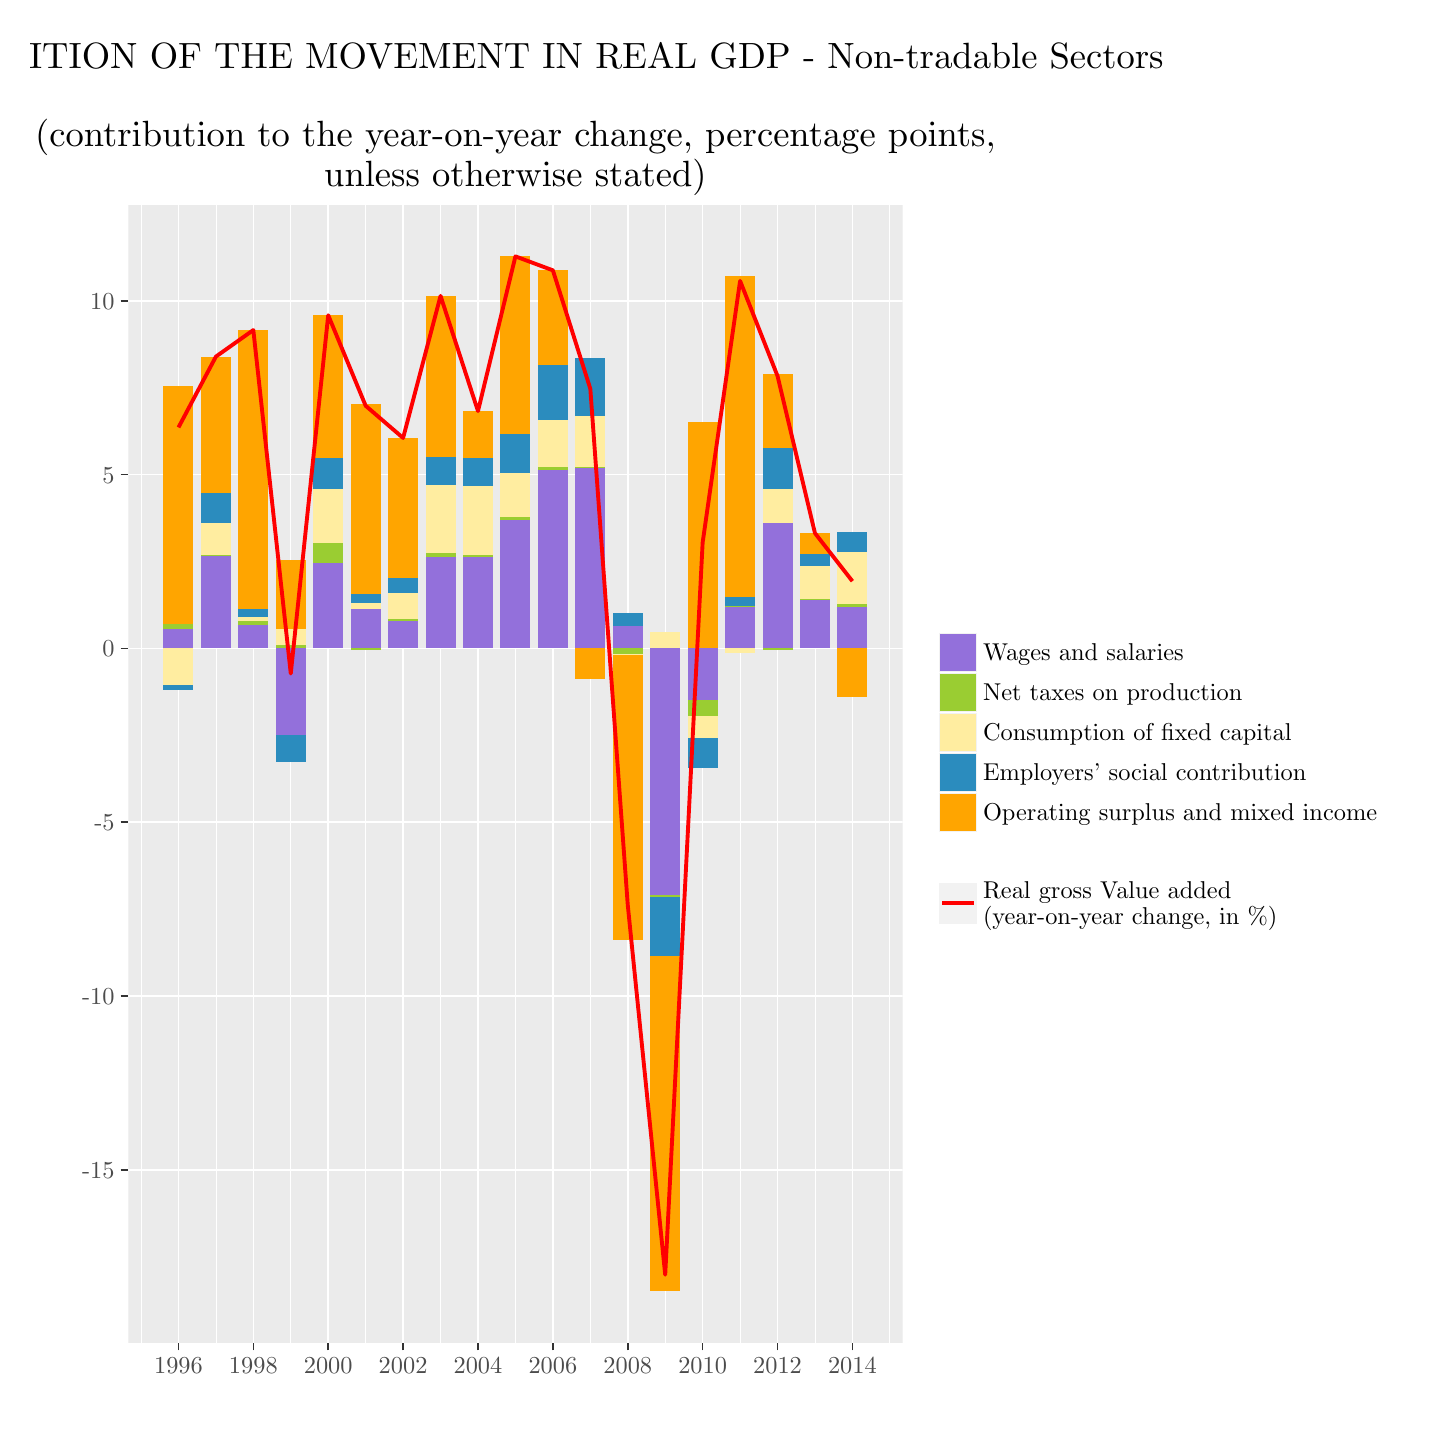
\begin{tikzpicture}[x=1pt,y=1pt]
\definecolor{fillColor}{RGB}{255,255,255}
\path[use as bounding box,fill=fillColor,fill opacity=0.00] (0,0) rectangle (505.89,505.89);
\begin{scope}
\path[clip] (  0.00,  0.00) rectangle (505.89,505.89);
\definecolor{drawColor}{RGB}{255,255,255}
\definecolor{fillColor}{RGB}{255,255,255}

\path[draw=drawColor,line width= 0.6pt,line join=round,line cap=round,fill=fillColor] (  0.00,  0.00) rectangle (505.89,505.89);
\end{scope}
\begin{scope}
\path[clip] ( 36.36, 30.69) rectangle (316.14,441.93);
\definecolor{fillColor}{gray}{0.92}

\path[fill=fillColor] ( 36.36, 30.69) rectangle (316.14,441.93);
\definecolor{drawColor}{RGB}{255,255,255}

\path[draw=drawColor,line width= 0.3pt,line join=round] ( 40.96, 30.69) --
	( 40.96,441.93);

\path[draw=drawColor,line width= 0.3pt,line join=round] ( 68.02, 30.69) --
	( 68.02,441.93);

\path[draw=drawColor,line width= 0.3pt,line join=round] ( 95.07, 30.69) --
	( 95.07,441.93);

\path[draw=drawColor,line width= 0.3pt,line join=round] (122.13, 30.69) --
	(122.13,441.93);

\path[draw=drawColor,line width= 0.3pt,line join=round] (149.19, 30.69) --
	(149.19,441.93);

\path[draw=drawColor,line width= 0.3pt,line join=round] (176.25, 30.69) --
	(176.25,441.93);

\path[draw=drawColor,line width= 0.3pt,line join=round] (203.31, 30.69) --
	(203.31,441.93);

\path[draw=drawColor,line width= 0.3pt,line join=round] (230.37, 30.69) --
	(230.37,441.93);

\path[draw=drawColor,line width= 0.3pt,line join=round] (257.43, 30.69) --
	(257.43,441.93);

\path[draw=drawColor,line width= 0.3pt,line join=round] (284.48, 30.69) --
	(284.48,441.93);

\path[draw=drawColor,line width= 0.3pt,line join=round] (311.54, 30.69) --
	(311.54,441.93);

\path[draw=drawColor,line width= 0.6pt,line join=round] ( 36.36, 93.14) --
	(316.14, 93.14);

\path[draw=drawColor,line width= 0.6pt,line join=round] ( 36.36,155.95) --
	(316.14,155.95);

\path[draw=drawColor,line width= 0.6pt,line join=round] ( 36.36,218.76) --
	(316.14,218.76);

\path[draw=drawColor,line width= 0.6pt,line join=round] ( 36.36,281.57) --
	(316.14,281.57);

\path[draw=drawColor,line width= 0.6pt,line join=round] ( 36.36,344.38) --
	(316.14,344.38);

\path[draw=drawColor,line width= 0.6pt,line join=round] ( 36.36,407.19) --
	(316.14,407.19);

\path[draw=drawColor,line width= 0.6pt,line join=round] ( 54.49, 30.69) --
	( 54.49,441.93);

\path[draw=drawColor,line width= 0.6pt,line join=round] ( 81.54, 30.69) --
	( 81.54,441.93);

\path[draw=drawColor,line width= 0.6pt,line join=round] (108.60, 30.69) --
	(108.60,441.93);

\path[draw=drawColor,line width= 0.6pt,line join=round] (135.66, 30.69) --
	(135.66,441.93);

\path[draw=drawColor,line width= 0.6pt,line join=round] (162.72, 30.69) --
	(162.72,441.93);

\path[draw=drawColor,line width= 0.6pt,line join=round] (189.78, 30.69) --
	(189.78,441.93);

\path[draw=drawColor,line width= 0.6pt,line join=round] (216.84, 30.69) --
	(216.84,441.93);

\path[draw=drawColor,line width= 0.6pt,line join=round] (243.90, 30.69) --
	(243.90,441.93);

\path[draw=drawColor,line width= 0.6pt,line join=round] (270.95, 30.69) --
	(270.95,441.93);

\path[draw=drawColor,line width= 0.6pt,line join=round] (298.01, 30.69) --
	(298.01,441.93);
\definecolor{fillColor}{RGB}{147,112,219}

\path[fill=fillColor] ( 49.07,281.57) rectangle ( 59.90,288.47);
\definecolor{fillColor}{RGB}{154,205,50}

\path[fill=fillColor] ( 49.07,288.47) rectangle ( 59.90,290.33);
\definecolor{fillColor}{RGB}{255,165,0}

\path[fill=fillColor] ( 49.07,290.33) rectangle ( 59.90,376.43);
\definecolor{fillColor}{RGB}{147,112,219}

\path[fill=fillColor] ( 62.60,281.57) rectangle ( 73.43,314.82);
\definecolor{fillColor}{RGB}{154,205,50}

\path[fill=fillColor] ( 62.60,314.82) rectangle ( 73.43,315.39);
\definecolor{fillColor}{RGB}{255,237,160}

\path[fill=fillColor] ( 62.60,315.39) rectangle ( 73.43,326.95);
\definecolor{fillColor}{RGB}{43,140,190}

\path[fill=fillColor] ( 62.60,326.95) rectangle ( 73.43,337.79);
\definecolor{fillColor}{RGB}{255,165,0}

\path[fill=fillColor] ( 62.60,337.79) rectangle ( 73.43,387.03);
\definecolor{fillColor}{RGB}{147,112,219}

\path[fill=fillColor] ( 76.13,281.57) rectangle ( 86.96,290.11);
\definecolor{fillColor}{RGB}{154,205,50}

\path[fill=fillColor] ( 76.13,290.11) rectangle ( 86.96,291.33);
\definecolor{fillColor}{RGB}{255,237,160}

\path[fill=fillColor] ( 76.13,291.33) rectangle ( 86.96,293.08);
\definecolor{fillColor}{RGB}{43,140,190}

\path[fill=fillColor] ( 76.13,293.08) rectangle ( 86.96,295.89);
\definecolor{fillColor}{RGB}{255,165,0}

\path[fill=fillColor] ( 76.13,295.89) rectangle ( 86.96,396.62);
\definecolor{fillColor}{RGB}{154,205,50}

\path[fill=fillColor] ( 89.66,281.57) rectangle (100.49,282.82);
\definecolor{fillColor}{RGB}{255,237,160}

\path[fill=fillColor] ( 89.66,282.82) rectangle (100.49,288.65);
\definecolor{fillColor}{RGB}{255,165,0}

\path[fill=fillColor] ( 89.66,288.65) rectangle (100.49,313.56);
\definecolor{fillColor}{RGB}{147,112,219}

\path[fill=fillColor] (103.19,281.57) rectangle (114.01,312.57);
\definecolor{fillColor}{RGB}{154,205,50}

\path[fill=fillColor] (103.19,312.57) rectangle (114.01,319.65);
\definecolor{fillColor}{RGB}{255,237,160}

\path[fill=fillColor] (103.19,319.65) rectangle (114.01,339.07);
\definecolor{fillColor}{RGB}{43,140,190}

\path[fill=fillColor] (103.19,339.07) rectangle (114.01,350.30);
\definecolor{fillColor}{RGB}{255,165,0}

\path[fill=fillColor] (103.19,350.30) rectangle (114.01,401.98);
\definecolor{fillColor}{RGB}{147,112,219}

\path[fill=fillColor] (116.72,281.57) rectangle (127.54,295.74);
\definecolor{fillColor}{RGB}{255,237,160}

\path[fill=fillColor] (116.72,295.74) rectangle (127.54,298.17);
\definecolor{fillColor}{RGB}{43,140,190}

\path[fill=fillColor] (116.72,298.17) rectangle (127.54,301.12);
\definecolor{fillColor}{RGB}{255,165,0}

\path[fill=fillColor] (116.72,301.12) rectangle (127.54,369.72);
\definecolor{fillColor}{RGB}{147,112,219}

\path[fill=fillColor] (130.25,281.57) rectangle (141.07,291.47);
\definecolor{fillColor}{RGB}{154,205,50}

\path[fill=fillColor] (130.25,291.47) rectangle (141.07,292.05);
\definecolor{fillColor}{RGB}{255,237,160}

\path[fill=fillColor] (130.25,292.05) rectangle (141.07,301.77);
\definecolor{fillColor}{RGB}{43,140,190}

\path[fill=fillColor] (130.25,301.77) rectangle (141.07,307.10);
\definecolor{fillColor}{RGB}{255,165,0}

\path[fill=fillColor] (130.25,307.10) rectangle (141.07,357.62);
\definecolor{fillColor}{RGB}{147,112,219}

\path[fill=fillColor] (143.78,281.57) rectangle (154.60,314.54);
\definecolor{fillColor}{RGB}{154,205,50}

\path[fill=fillColor] (143.78,314.54) rectangle (154.60,316.19);
\definecolor{fillColor}{RGB}{255,237,160}

\path[fill=fillColor] (143.78,316.19) rectangle (154.60,340.80);
\definecolor{fillColor}{RGB}{43,140,190}

\path[fill=fillColor] (143.78,340.80) rectangle (154.60,350.72);
\definecolor{fillColor}{RGB}{255,165,0}

\path[fill=fillColor] (143.78,350.72) rectangle (154.60,408.96);
\definecolor{fillColor}{RGB}{147,112,219}

\path[fill=fillColor] (157.31,281.57) rectangle (168.13,314.77);
\definecolor{fillColor}{RGB}{154,205,50}

\path[fill=fillColor] (157.31,314.77) rectangle (168.13,315.47);
\definecolor{fillColor}{RGB}{255,237,160}

\path[fill=fillColor] (157.31,315.47) rectangle (168.13,340.43);
\definecolor{fillColor}{RGB}{43,140,190}

\path[fill=fillColor] (157.31,340.43) rectangle (168.13,350.41);
\definecolor{fillColor}{RGB}{255,165,0}

\path[fill=fillColor] (157.31,350.41) rectangle (168.13,367.33);
\definecolor{fillColor}{RGB}{147,112,219}

\path[fill=fillColor] (170.84,281.57) rectangle (181.66,327.85);
\definecolor{fillColor}{RGB}{154,205,50}

\path[fill=fillColor] (170.84,327.85) rectangle (181.66,329.19);
\definecolor{fillColor}{RGB}{255,237,160}

\path[fill=fillColor] (170.84,329.19) rectangle (181.66,344.92);
\definecolor{fillColor}{RGB}{43,140,190}

\path[fill=fillColor] (170.84,344.92) rectangle (181.66,358.95);
\definecolor{fillColor}{RGB}{255,165,0}

\path[fill=fillColor] (170.84,358.95) rectangle (181.66,423.24);
\definecolor{fillColor}{RGB}{147,112,219}

\path[fill=fillColor] (184.37,281.57) rectangle (195.19,346.21);
\definecolor{fillColor}{RGB}{154,205,50}

\path[fill=fillColor] (184.37,346.21) rectangle (195.19,347.22);
\definecolor{fillColor}{RGB}{255,237,160}

\path[fill=fillColor] (184.37,347.22) rectangle (195.19,364.21);
\definecolor{fillColor}{RGB}{43,140,190}

\path[fill=fillColor] (184.37,364.21) rectangle (195.19,383.87);
\definecolor{fillColor}{RGB}{255,165,0}

\path[fill=fillColor] (184.37,383.87) rectangle (195.19,418.20);
\definecolor{fillColor}{RGB}{147,112,219}

\path[fill=fillColor] (197.90,281.57) rectangle (208.72,346.60);
\definecolor{fillColor}{RGB}{154,205,50}

\path[fill=fillColor] (197.90,346.60) rectangle (208.72,347.29);
\definecolor{fillColor}{RGB}{255,237,160}

\path[fill=fillColor] (197.90,347.29) rectangle (208.72,365.58);
\definecolor{fillColor}{RGB}{43,140,190}

\path[fill=fillColor] (197.90,365.58) rectangle (208.72,386.47);
\definecolor{fillColor}{RGB}{147,112,219}

\path[fill=fillColor] (211.43,281.57) rectangle (222.25,289.58);
\definecolor{fillColor}{RGB}{43,140,190}

\path[fill=fillColor] (211.43,289.58) rectangle (222.25,294.34);
\definecolor{fillColor}{RGB}{255,237,160}

\path[fill=fillColor] (224.95,281.57) rectangle (235.78,287.45);
\definecolor{fillColor}{RGB}{255,165,0}

\path[fill=fillColor] (238.48,281.57) rectangle (249.31,363.22);
\definecolor{fillColor}{RGB}{147,112,219}

\path[fill=fillColor] (252.01,281.57) rectangle (262.84,296.53);
\definecolor{fillColor}{RGB}{154,205,50}

\path[fill=fillColor] (252.01,296.53) rectangle (262.84,296.97);
\definecolor{fillColor}{RGB}{43,140,190}

\path[fill=fillColor] (252.01,296.97) rectangle (262.84,300.06);
\definecolor{fillColor}{RGB}{255,165,0}

\path[fill=fillColor] (252.01,300.06) rectangle (262.84,416.01);
\definecolor{fillColor}{RGB}{147,112,219}

\path[fill=fillColor] (265.54,281.57) rectangle (276.37,326.91);
\definecolor{fillColor}{RGB}{255,237,160}

\path[fill=fillColor] (265.54,326.91) rectangle (276.37,339.15);
\definecolor{fillColor}{RGB}{43,140,190}

\path[fill=fillColor] (265.54,339.15) rectangle (276.37,354.15);
\definecolor{fillColor}{RGB}{255,165,0}

\path[fill=fillColor] (265.54,354.15) rectangle (276.37,380.64);
\definecolor{fillColor}{RGB}{147,112,219}

\path[fill=fillColor] (279.07,281.57) rectangle (289.90,299.17);
\definecolor{fillColor}{RGB}{154,205,50}

\path[fill=fillColor] (279.07,299.17) rectangle (289.90,299.28);
\definecolor{fillColor}{RGB}{255,237,160}

\path[fill=fillColor] (279.07,299.28) rectangle (289.90,311.22);
\definecolor{fillColor}{RGB}{43,140,190}

\path[fill=fillColor] (279.07,311.22) rectangle (289.90,315.86);
\definecolor{fillColor}{RGB}{255,165,0}

\path[fill=fillColor] (279.07,315.86) rectangle (289.90,323.24);
\definecolor{fillColor}{RGB}{147,112,219}

\path[fill=fillColor] (292.60,281.57) rectangle (303.42,296.57);
\definecolor{fillColor}{RGB}{154,205,50}

\path[fill=fillColor] (292.60,296.57) rectangle (303.42,297.78);
\definecolor{fillColor}{RGB}{255,237,160}

\path[fill=fillColor] (292.60,297.78) rectangle (303.42,316.42);
\definecolor{fillColor}{RGB}{43,140,190}

\path[fill=fillColor] (292.60,316.42) rectangle (303.42,323.51);
\definecolor{fillColor}{RGB}{255,237,160}

\path[fill=fillColor] ( 49.07,281.57) rectangle ( 59.90,268.24);
\definecolor{fillColor}{RGB}{43,140,190}

\path[fill=fillColor] ( 49.07,268.24) rectangle ( 59.90,266.58);
\definecolor{fillColor}{RGB}{147,112,219}

\path[fill=fillColor] ( 89.66,281.57) rectangle (100.49,250.43);
\definecolor{fillColor}{RGB}{43,140,190}

\path[fill=fillColor] ( 89.66,250.43) rectangle (100.49,240.51);
\definecolor{fillColor}{RGB}{154,205,50}

\path[fill=fillColor] (116.72,281.12) rectangle (127.54,281.57);
\definecolor{fillColor}{RGB}{255,165,0}

\path[fill=fillColor] (197.90,270.52) rectangle (208.72,281.57);
\definecolor{fillColor}{RGB}{154,205,50}

\path[fill=fillColor] (211.43,281.57) rectangle (222.25,279.42);
\definecolor{fillColor}{RGB}{255,237,160}

\path[fill=fillColor] (211.43,279.42) rectangle (222.25,279.34);
\definecolor{fillColor}{RGB}{255,165,0}

\path[fill=fillColor] (211.43,279.34) rectangle (222.25,176.10);
\definecolor{fillColor}{RGB}{147,112,219}

\path[fill=fillColor] (224.95,281.57) rectangle (235.78,192.53);
\definecolor{fillColor}{RGB}{154,205,50}

\path[fill=fillColor] (224.95,192.53) rectangle (235.78,191.80);
\definecolor{fillColor}{RGB}{43,140,190}

\path[fill=fillColor] (224.95,191.80) rectangle (235.78,170.46);
\definecolor{fillColor}{RGB}{255,165,0}

\path[fill=fillColor] (224.95,170.46) rectangle (235.78, 49.38);
\definecolor{fillColor}{RGB}{147,112,219}

\path[fill=fillColor] (238.48,281.57) rectangle (249.31,262.99);
\definecolor{fillColor}{RGB}{154,205,50}

\path[fill=fillColor] (238.48,262.99) rectangle (249.31,257.15);
\definecolor{fillColor}{RGB}{255,237,160}

\path[fill=fillColor] (238.48,257.15) rectangle (249.31,249.36);
\definecolor{fillColor}{RGB}{43,140,190}

\path[fill=fillColor] (238.48,249.36) rectangle (249.31,238.22);
\definecolor{fillColor}{RGB}{255,237,160}

\path[fill=fillColor] (252.01,279.96) rectangle (262.84,281.57);
\definecolor{fillColor}{RGB}{154,205,50}

\path[fill=fillColor] (265.54,280.97) rectangle (276.37,281.57);
\definecolor{fillColor}{RGB}{255,165,0}

\path[fill=fillColor] (292.60,263.93) rectangle (303.42,281.57);
\definecolor{drawColor}{RGB}{255,0,0}

\path[draw=drawColor,line width= 1.4pt,line join=round] ( 54.49,361.43) --
	( 68.02,387.03) --
	( 81.54,396.62) --
	( 95.07,272.50) --
	(108.60,401.98) --
	(122.13,369.26) --
	(135.66,357.62) --
	(149.19,408.96) --
	(162.72,367.33) --
	(176.25,423.24) --
	(189.78,418.20) --
	(203.31,375.41) --
	(216.84,188.87) --
	(230.37, 55.25) --
	(243.90,319.86) --
	(257.43,414.39) --
	(270.95,380.04) --
	(284.48,323.24) --
	(298.01,305.87);
\end{scope}
\begin{scope}
\path[clip] (  0.00,  0.00) rectangle (505.89,505.89);
\definecolor{drawColor}{gray}{0.30}

\node[text=drawColor,anchor=base east,inner sep=0pt, outer sep=0pt, scale=  0.88] at ( 31.41, 90.11) {-15};

\node[text=drawColor,anchor=base east,inner sep=0pt, outer sep=0pt, scale=  0.88] at ( 31.41,152.92) {-10};

\node[text=drawColor,anchor=base east,inner sep=0pt, outer sep=0pt, scale=  0.88] at ( 31.41,215.73) {-5};

\node[text=drawColor,anchor=base east,inner sep=0pt, outer sep=0pt, scale=  0.88] at ( 31.41,278.54) {0};

\node[text=drawColor,anchor=base east,inner sep=0pt, outer sep=0pt, scale=  0.88] at ( 31.41,341.35) {5};

\node[text=drawColor,anchor=base east,inner sep=0pt, outer sep=0pt, scale=  0.88] at ( 31.41,404.16) {10};
\end{scope}
\begin{scope}
\path[clip] (  0.00,  0.00) rectangle (505.89,505.89);
\definecolor{drawColor}{gray}{0.20}

\path[draw=drawColor,line width= 0.6pt,line join=round] ( 33.61, 93.14) --
	( 36.36, 93.14);

\path[draw=drawColor,line width= 0.6pt,line join=round] ( 33.61,155.95) --
	( 36.36,155.95);

\path[draw=drawColor,line width= 0.6pt,line join=round] ( 33.61,218.76) --
	( 36.36,218.76);

\path[draw=drawColor,line width= 0.6pt,line join=round] ( 33.61,281.57) --
	( 36.36,281.57);

\path[draw=drawColor,line width= 0.6pt,line join=round] ( 33.61,344.38) --
	( 36.36,344.38);

\path[draw=drawColor,line width= 0.6pt,line join=round] ( 33.61,407.19) --
	( 36.36,407.19);
\end{scope}
\begin{scope}
\path[clip] (  0.00,  0.00) rectangle (505.89,505.89);
\definecolor{drawColor}{gray}{0.20}

\path[draw=drawColor,line width= 0.6pt,line join=round] ( 54.49, 27.94) --
	( 54.49, 30.69);

\path[draw=drawColor,line width= 0.6pt,line join=round] ( 81.54, 27.94) --
	( 81.54, 30.69);

\path[draw=drawColor,line width= 0.6pt,line join=round] (108.60, 27.94) --
	(108.60, 30.69);

\path[draw=drawColor,line width= 0.6pt,line join=round] (135.66, 27.94) --
	(135.66, 30.69);

\path[draw=drawColor,line width= 0.6pt,line join=round] (162.72, 27.94) --
	(162.72, 30.69);

\path[draw=drawColor,line width= 0.6pt,line join=round] (189.78, 27.94) --
	(189.78, 30.69);

\path[draw=drawColor,line width= 0.6pt,line join=round] (216.84, 27.94) --
	(216.84, 30.69);

\path[draw=drawColor,line width= 0.6pt,line join=round] (243.90, 27.94) --
	(243.90, 30.69);

\path[draw=drawColor,line width= 0.6pt,line join=round] (270.95, 27.94) --
	(270.95, 30.69);

\path[draw=drawColor,line width= 0.6pt,line join=round] (298.01, 27.94) --
	(298.01, 30.69);
\end{scope}
\begin{scope}
\path[clip] (  0.00,  0.00) rectangle (505.89,505.89);
\definecolor{drawColor}{gray}{0.30}

\node[text=drawColor,anchor=base,inner sep=0pt, outer sep=0pt, scale=  0.88] at ( 54.49, 19.68) {1996};

\node[text=drawColor,anchor=base,inner sep=0pt, outer sep=0pt, scale=  0.88] at ( 81.54, 19.68) {1998};

\node[text=drawColor,anchor=base,inner sep=0pt, outer sep=0pt, scale=  0.88] at (108.60, 19.68) {2000};

\node[text=drawColor,anchor=base,inner sep=0pt, outer sep=0pt, scale=  0.88] at (135.66, 19.68) {2002};

\node[text=drawColor,anchor=base,inner sep=0pt, outer sep=0pt, scale=  0.88] at (162.72, 19.68) {2004};

\node[text=drawColor,anchor=base,inner sep=0pt, outer sep=0pt, scale=  0.88] at (189.78, 19.68) {2006};

\node[text=drawColor,anchor=base,inner sep=0pt, outer sep=0pt, scale=  0.88] at (216.84, 19.68) {2008};

\node[text=drawColor,anchor=base,inner sep=0pt, outer sep=0pt, scale=  0.88] at (243.90, 19.68) {2010};

\node[text=drawColor,anchor=base,inner sep=0pt, outer sep=0pt, scale=  0.88] at (270.95, 19.68) {2012};

\node[text=drawColor,anchor=base,inner sep=0pt, outer sep=0pt, scale=  0.88] at (298.01, 19.68) {2014};
\end{scope}
\begin{scope}
\path[clip] (  0.00,  0.00) rectangle (505.89,505.89);
\definecolor{fillColor}{RGB}{255,255,255}

\path[fill=fillColor] (324.68,210.80) rectangle (491.85,295.22);
\end{scope}
\begin{scope}
\path[clip] (  0.00,  0.00) rectangle (505.89,505.89);
\definecolor{drawColor}{RGB}{255,255,255}
\definecolor{fillColor}{gray}{0.95}

\path[draw=drawColor,line width= 0.6pt,line join=round,line cap=round,fill=fillColor] (328.95,272.89) rectangle (343.40,287.34);
\end{scope}
\begin{scope}
\path[clip] (  0.00,  0.00) rectangle (505.89,505.89);
\definecolor{fillColor}{RGB}{147,112,219}

\path[fill=fillColor] (329.66,273.60) rectangle (342.69,286.63);
\end{scope}
\begin{scope}
\path[clip] (  0.00,  0.00) rectangle (505.89,505.89);
\definecolor{fillColor}{RGB}{147,112,219}

\path[fill=fillColor] (329.66,273.60) rectangle (342.69,286.63);
\end{scope}
\begin{scope}
\path[clip] (  0.00,  0.00) rectangle (505.89,505.89);
\definecolor{drawColor}{RGB}{255,255,255}
\definecolor{fillColor}{gray}{0.95}

\path[draw=drawColor,line width= 0.6pt,line join=round,line cap=round,fill=fillColor] (328.95,258.43) rectangle (343.40,272.89);
\end{scope}
\begin{scope}
\path[clip] (  0.00,  0.00) rectangle (505.89,505.89);
\definecolor{fillColor}{RGB}{154,205,50}

\path[fill=fillColor] (329.66,259.14) rectangle (342.69,272.17);
\end{scope}
\begin{scope}
\path[clip] (  0.00,  0.00) rectangle (505.89,505.89);
\definecolor{fillColor}{RGB}{154,205,50}

\path[fill=fillColor] (329.66,259.14) rectangle (342.69,272.17);
\end{scope}
\begin{scope}
\path[clip] (  0.00,  0.00) rectangle (505.89,505.89);
\definecolor{drawColor}{RGB}{255,255,255}
\definecolor{fillColor}{gray}{0.95}

\path[draw=drawColor,line width= 0.6pt,line join=round,line cap=round,fill=fillColor] (328.95,243.98) rectangle (343.40,258.43);
\end{scope}
\begin{scope}
\path[clip] (  0.00,  0.00) rectangle (505.89,505.89);
\definecolor{fillColor}{RGB}{255,237,160}

\path[fill=fillColor] (329.66,244.69) rectangle (342.69,257.72);
\end{scope}
\begin{scope}
\path[clip] (  0.00,  0.00) rectangle (505.89,505.89);
\definecolor{fillColor}{RGB}{255,237,160}

\path[fill=fillColor] (329.66,244.69) rectangle (342.69,257.72);
\end{scope}
\begin{scope}
\path[clip] (  0.00,  0.00) rectangle (505.89,505.89);
\definecolor{drawColor}{RGB}{255,255,255}
\definecolor{fillColor}{gray}{0.95}

\path[draw=drawColor,line width= 0.6pt,line join=round,line cap=round,fill=fillColor] (328.95,229.52) rectangle (343.40,243.98);
\end{scope}
\begin{scope}
\path[clip] (  0.00,  0.00) rectangle (505.89,505.89);
\definecolor{fillColor}{RGB}{43,140,190}

\path[fill=fillColor] (329.66,230.23) rectangle (342.69,243.27);
\end{scope}
\begin{scope}
\path[clip] (  0.00,  0.00) rectangle (505.89,505.89);
\definecolor{fillColor}{RGB}{43,140,190}

\path[fill=fillColor] (329.66,230.23) rectangle (342.69,243.27);
\end{scope}
\begin{scope}
\path[clip] (  0.00,  0.00) rectangle (505.89,505.89);
\definecolor{drawColor}{RGB}{255,255,255}
\definecolor{fillColor}{gray}{0.95}

\path[draw=drawColor,line width= 0.6pt,line join=round,line cap=round,fill=fillColor] (328.95,215.07) rectangle (343.40,229.52);
\end{scope}
\begin{scope}
\path[clip] (  0.00,  0.00) rectangle (505.89,505.89);
\definecolor{fillColor}{RGB}{255,165,0}

\path[fill=fillColor] (329.66,215.78) rectangle (342.69,228.81);
\end{scope}
\begin{scope}
\path[clip] (  0.00,  0.00) rectangle (505.89,505.89);
\definecolor{fillColor}{RGB}{255,165,0}

\path[fill=fillColor] (329.66,215.78) rectangle (342.69,228.81);
\end{scope}
\begin{scope}
\path[clip] (  0.00,  0.00) rectangle (505.89,505.89);
\definecolor{drawColor}{RGB}{0,0,0}

\node[text=drawColor,anchor=base west,inner sep=0pt, outer sep=0pt, scale=  0.88] at (345.21,277.08) {Wages and salaries};
\end{scope}
\begin{scope}
\path[clip] (  0.00,  0.00) rectangle (505.89,505.89);
\definecolor{drawColor}{RGB}{0,0,0}

\node[text=drawColor,anchor=base west,inner sep=0pt, outer sep=0pt, scale=  0.88] at (345.21,262.63) {Net taxes on production};
\end{scope}
\begin{scope}
\path[clip] (  0.00,  0.00) rectangle (505.89,505.89);
\definecolor{drawColor}{RGB}{0,0,0}

\node[text=drawColor,anchor=base west,inner sep=0pt, outer sep=0pt, scale=  0.88] at (345.21,248.17) {Consumption of fixed capital};
\end{scope}
\begin{scope}
\path[clip] (  0.00,  0.00) rectangle (505.89,505.89);
\definecolor{drawColor}{RGB}{0,0,0}

\node[text=drawColor,anchor=base west,inner sep=0pt, outer sep=0pt, scale=  0.88] at (345.21,233.72) {Employers' social contribution};
\end{scope}
\begin{scope}
\path[clip] (  0.00,  0.00) rectangle (505.89,505.89);
\definecolor{drawColor}{RGB}{0,0,0}

\node[text=drawColor,anchor=base west,inner sep=0pt, outer sep=0pt, scale=  0.88] at (345.21,219.27) {Operating surplus and mixed income};
\end{scope}
\begin{scope}
\path[clip] (  0.00,  0.00) rectangle (505.89,505.89);
\definecolor{fillColor}{RGB}{255,255,255}

\path[fill=fillColor] (324.68,177.40) rectangle (455.83,205.11);
\end{scope}
\begin{scope}
\path[clip] (  0.00,  0.00) rectangle (505.89,505.89);
\definecolor{drawColor}{RGB}{255,255,255}
\definecolor{fillColor}{gray}{0.95}

\path[draw=drawColor,line width= 0.6pt,line join=round,line cap=round,fill=fillColor] (328.95,181.66) rectangle (343.40,197.23);
\end{scope}
\begin{scope}
\path[clip] (  0.00,  0.00) rectangle (505.89,505.89);
\definecolor{drawColor}{RGB}{255,0,0}

\path[draw=drawColor,line width= 1.4pt,line join=round] (330.39,189.45) -- (341.95,189.45);
\end{scope}
\begin{scope}
\path[clip] (  0.00,  0.00) rectangle (505.89,505.89);
\definecolor{drawColor}{RGB}{0,0,0}

\node[text=drawColor,anchor=base west,inner sep=0pt, outer sep=0pt, scale=  0.88] at (345.21,191.17) {Real gross Value added };

\node[text=drawColor,anchor=base west,inner sep=0pt, outer sep=0pt, scale=  0.88] at (345.21,181.66) {(year-on-year change, in {\%})};
\end{scope}
\begin{scope}
\path[clip] (  0.00,  0.00) rectangle (505.89,505.89);
\definecolor{drawColor}{RGB}{0,0,0}

\node[text=drawColor,anchor=base,inner sep=0pt, outer sep=0pt, scale=  1.32] at (176.25,491.30) {COMPOSITION OF THE MOVEMENT IN REAL GDP - Non-tradable Sectors};

\node[text=drawColor,anchor=base,inner sep=0pt, outer sep=0pt, scale=  1.32] at (176.25,477.04) {          };

\node[text=drawColor,anchor=base,inner sep=0pt, outer sep=0pt, scale=  1.32] at (176.25,462.79) {(contribution to the year-on-year change, percentage points,};

\node[text=drawColor,anchor=base,inner sep=0pt, outer sep=0pt, scale=  1.32] at (176.25,448.53) {          unless otherwise stated)};
\end{scope}
\end{tikzpicture}
